\documentclass[../main.tex]{subfiles}
\begin{document}
\subsection{Условие применимости метода линеаризации в задаче локального синтеза} 
Этот раздел посвящен задаче синтеза обратной связи для нелинейной аффинной по управлению системы. 
Целью управления является приведение траектории замкнутой системы в начало координат. 
Объектом изучения является нелинейная система, замкнутая линейной обратной связью. 
Эта обратная связь является решением линейно-квадратичной задачи для линеаризованной системы. 
Мы приводим достаточные условия, при выполнении которых эта обратная связь дает локальное решение рассматриваемой задачи управления.  
Также приводятся некоторые оценки значений интегрального функционала.  

Раздел организован следующим образом. 
В первом подразделе приводится формулировка задачи и некоторые предварительные результаты. 
Во втором подразделе 
Следующий подраздел содержит результаты, относящиеся к асимптотике траекторий нелинейной системы, замкнутой линейной обратной связью. 
Четвертый подраздел посвящен оценке погрешностей в значении функционала при использовании линейной обратной связи. 
Наконец, в последнем подразделе приведены два иллюстративных примера.

\subsubsection{Постановка задачи}

Рассмотрим нелинейную систему, аффинную по управлению
\begin{gather}\label{sec22:nonlinear}
	\dot{z}(t)=f(z(t))+B u(t),\qquad 0 \leqslant t \leqslant T, \qquad z(0) = z_0.
\end{gather}
 где $ x \in \mathbb{R}^n $ --- вектор состояния, $ u \in \mathbb{R}^r $ --- вектор управления, а $ 
T$ --- некоторое положительное число. 
Будем считать, что функция $f$ обладает следующим свойством.
\begin{property}\label{prop:Residial_term_bounds}
	 Найдутся такие  $r>0$, $k>0$  что при всех $ z \in B(0,r) $, функция  $f(z)$ может быть представлена в форме  $ f(z) = Az + R(z) $, причем  $ \|R(z) \| \leqslant k \| z\|^2  $. 
\end{property}
Здесь $ B(0,r) $ --- это шар радиуса $r$  с центром в точке $0 \in \mathbb{R}^n$. 
Это свойство выполняется, если if $f(0) = 0 $, $\frac{\partial f}{\partial x}(0) 
= A $ и $f(z)$ дважды дифференцируема. 

Напомним, что пространство скалярных или векторных функций интегрируемых с квадратом  на $ [0,T] $ обозначаются через $ \mathbb{L}_2 = \mathbb{L}_2[0,T] $. Шар в пространстве $\mathbb{L}_2$ обозначим через $B_{\mathbb{L}_2}(0,r)$. В качестве функционала мы рассматриваем 
\begin{gather}\label{cost}
		I(T,u):=\int_0^Tu^\top (t)u(t)dt= 	\lVert u(\cdot)\rVert^2_{\mathbb{L}_2.} 
\end{gather}
Задача состоит в синтезе закона управления $u(t)=u(t,z(t))$ который бы приводил траектории замкнутой системы  
\begin{gather*}
	\dot{z}(t)=f(z(t))+B u(t,z(t)),\qquad 0 \leqslant t \leqslant T, \qquad z(0) = z_0.
\end{gather*}
в начало координат за время $T$ и обеспечивал при этом минимальное значение $I(T,u)$. 

Рассмотрим линейный случай ($R(z)=0$)
\begin{gather}\label{sec22:linear}
	\dot{z} =  A  z + B u, \qquad 0 \leqslant t \leqslant T.
\end{gather}
Если система \eqref{sec22:linear} управляема, то решение описанной выше задачи --- это линейный по состоянию закон управления 
\begin{gather}\label{linear_feedback}
	u(t,z) = -B^{\top} Q_T(t) z
\end{gather}
(см, например, \cite{Abgar,Kur1,GusevOsipov}).
Здесь $Q_T(t)=W^{-1}(T-t)$, а $W(t)$ --- грамиан управляемости системы $\dot{x} = -A x - B u$:
\begin{gather*}
    W(t) = \int_0^t e^{-A\tau}BB^\top e^{-A^{\top}\tau}d\tau. 
\end{gather*}
Грамиан $W(t)$ положительно определен при $t>0$ тогда и только того, когда   
система \eqref{sec22:linear} управляема. Можно показать, что $Q_T(t)$ --- решение дифференциального уравнения 
\begin{gather}\label{eqQ}
	\dot{Q_T}  = Q_T B B^{\top} Q_T - A^{\top}Q_T - Q_T A, \quad Q_T(0)=W^{-1}(T).
\end{gather}
Таким образом, чтобы найти $Q_T(t)$ на $(0,T]$, нужно сначала вычислить $W(T)$, а затем проинтегрировать систему \eqref{eqQ}.
Поскольку $W(0)=0$, $Q_T(t)$ определена для $t<T$ и $\|Q_T(t)\| \to \infty$ при $t\to T$. 

Верно следующее утверждение \cite{Abgar,Kur1,GusevOsipov}.
\begin{utv}
Любая траектория $z(t)$ системы \eqref{sec22:linear} с управлением  \eqref{linear_feedback} выходящая из точки  $ z_0 $ достигает начала координат за время $T$. При этом интегральный функционал $I(T,u)$ принимает минимальное значение $z^{\top}_0 Q_T(0) z_0 $ при каждом $z_0$.
\end{utv}
Далее мы будем исследовать поведение траекторий системы \eqref{sec22:nonlinear} замкнутой линейной обратной связью $ u(t,z) = -B^{\top} Q_T(t) z$ при условии, что  $T$ достаточно мало. 
Верно ли, что все траектории, начинающиеся в некоторой окрестности начала координат, достигают его?  
Можно ли что-то сказать о значении интегрального функционала? 

\subsubsection{Асимптотическая эквивалентность множеств достижимости}

Далее, мы будем использовать понятие асимптотической эквивалентности множеств, введенное в разделе \ref{sec21:AsymptoticEquality}. 
Рассмотрим систему, уравнения которой получаются из \eqref{sec22:nonlinear} обращением времени. Положив $\tau=T-t$ мы имеем
\begin{gather}\label{nonlinear_}
			\dot{x}(\tau)=-f(x(\tau))-B v(\tau),\qquad 0 \leqslant \tau \leqslant T; 
\end{gather}
здесь $x(\tau)=z(T-\tau)$, $v(\tau)=u(T-\tau)$.
При заданном $\mu>0$ обозначим через $ G_{-} (T,\mu)$ множество достижимости системы \eqref{nonlinear_} с интегральными квадратичными ограничениями на управление, $G_{-}(T,\mu)=\{x\in \mathbb{R}^n:\exists v(\cdot)\in B_{\mathbb{L}_2}(0,\mu),\; x=x( T,v(\cdot)))\}$.
		 
Здесь $x( \tau,v(\cdot)))$ обозначает решение системы  \eqref{nonlinear_} с нулевыми начальными условиями. 
Свойства множеств достижимости нелинейных систем с интегральными ограничениями на управление изучались во многих работах (см., например, \cite{Guseinov,Rousse,GusZykIFAC}).
Рассмотрим также линейную систему 
\begin{gather}\label{linear_}
			\dot{x}(\tau)=-Ax(\tau)-B v(\tau),\qquad 0 \leqslant \tau \leqslant T; 
\end{gather}
эта система является линеаризацией системы  \eqref{nonlinear_} в начале координат. 
Множество достижимости этой системы обозначим через $G_{-}^0(T,\mu)$. 
Это множество --- эллипсоид в $\mathbb{R}^n$, описываемый неравенством $G_{-}^0(T,\mu)=\{x \in \mathbb{R}^n: x^\top W^{-1}(T)x\leqslant \mu^2\}$.			

%Let $X,Y \subset \mathbb R^n $ be convex compact sets such that the origin is an interior point of both the sets.
%\begin{definition}[see, for example, \cite{Lassak,Ovs}]
%The Banach-Mazur distance between $X$ and $Y$  is defined as
%$\rho(X,Y):=\log\big(r(X,Y)\cdot r(Y,X)\big)$, where \\ $r(X,Y)=\inf \{t\geqslant1:tX \supset Y\}$. 
%\end{definition} 
%From the definition it follows that for any $c>0$, $\rho(cX,cY)=\rho(X,Y)$ and two inclusions are valid: $X\subset \exp(\rho(X,Y))Y$ and $Y\subset \exp(\rho(X,Y))X$.

%Assume that  $X,Y$ depend on a small positive parameter $\tau$,  $0<\tau\leqslant\tau_0$  and set-valued mappings  $X(\tau), Y(\tau)$ are bounded. 
%\begin{definition}[\cite{Ovs}]	
% The sets $ X (\tau), Y (\tau) $ are called asymptotically equal under $\tau \to 0$ if $ \rho (X (\tau), Y (\tau)) \to 0,\;\; \tau \to 0$.
%\end{definition}
Через $\nu(\tau), \eta(\tau)$ обозначим наименьшее и наибольшее собственное число $W(\tau)$ соответственно. Из результатов  \cite{Polyak2001,GusOsSteklov,Osipov,GusevMotor} следует, что множества достижимости  
$G_{-}(\tau,\mu)$ и $G_{-}^0(\tau,\mu)$ асимптотически эквивалентны при $\tau \to 0$ если пара  $(A,B)$ --- управляема 
и существуют такие $ l > 0$, $\tau_0 > 0$ и $\alpha > 0$ что для всех $0 < \tau \leqslant \tau_0 $
		\begin{gather}\label{gramas}
			\nu(\tau)\geqslant l\tau^{4-\alpha}.
		\end{gather}

\begin{zam}
    Множество достижимости $G_{-}(T,\mu)$ системы \eqref{nonlinear_} совпадает с множеством нуль-\\-управляемости системы \eqref{sec22:nonlinear}, т.е. множества таких начальных условий, из которых система может быть переведена в начало координат управлениями из $B_{\mathbb{L}_2}(0,\mu) $ за время $T$. 
    То же самое справедливо для систем \eqref{linear_} и \eqref{linear_} и соответствующих им множеств $G_{-}^0(T,\mu)$.
\end{zam}

\subsubsection{Задача синтеза управления. Асимптотика траекторий}

Далее мы будем предполагать, что пара $A,/ B$ является управляемой, не уточняя это отдельно.

В этом разделе мы исследуем асимптотическое поведение траекторий системы \eqref{sec22:nonlinear}, замкнутой линейной обратной связью $ u(t,z) = -B^{\top} Q_T(t) z$:
\begin{equation}\label{nonlinear_closed}
	\dot{z} = f(z) - B B^{\top} Q_T(t) z, \qquad 0 \leqslant t \leqslant T, \qquad z(0) = z_0.
\end{equation}
Напомним, что это управление приводит траектории линейной системы $\dot{z} = A z + B z$ к началу координат в момент времени $T$ и обеспечивает минимальное значение функционала. 
Это значение равно $J_0(T,z_0) =z_0^{\top}Q_T(0)z_0$.

Для анализа траекторий системы \eqref{nonlinear_closed} используем следующую лемму
\begin{lemma}\label{lem:zqz} 
    Пусть $C\in \mathbb{R}^{ n \times n}$ и $D\in \mathbb{R}^{n \times n}$ --- симметричные положительно-определенные матрицы, $C=D^{-1}$. Тогда, для любого $\forall z \in \mathbb{R}^{n}$   
    \begin{gather} \label{eig}
        \frac{1}{\lambda_{max}(D)} \|z\|^2 \leqslant z^T C z \leqslant \frac{1}{\lambda_{min}(D)} \|z\|^2,
    \end{gather}
    где $\lambda_{max}(D)$ и $\lambda_{min}(D)$ --- наибольшее и наименьшее собственное число матрицы $D$.
\end{lemma}
\doc. 
  Следует из факта, что наибольшее и наименьшее собственное число матрицы $C$ равны $1/{\lambda_{min}(D)}$ и $1/{\lambda_{max}(D)}$, соответственно. \hfill $ \square $

Если $C=Q_T(t)=W^{-1}(T-t)$, то $D=W(T-t)$ и неравенство \eqref{eig} принимает вид
\begin{gather*} %\label{eig1}
        \frac{1}{\eta(T-t)} \|z\|^2 \leqslant z^T Q_T(t) z \leqslant \frac{1}{\nu(T-t)} \|z\|^2, \quad 0\leqslant t < T.
    \end{gather*}
\begin{assumption} \label{asm1}   
   Пусть существует $\overline{T}>0$ и непрерывная положительная функция $\varphi(\tau): (0, \overline{T}] \to \mathbb{R}$ такие, что
\begin{equation*}
    0 < \frac{\eta(\tau)}{\sqrt{\nu(\tau)}} \leqslant \varphi(\tau), \qquad 0 < \tau \leqslant \overline{T},\quad \int\limits_0^ {\overline{T}}\varphi(\tau) d\tau<\infty.
\end{equation*} 
\end{assumption}
Введем функцию $\Phi(T): [0, \overline{T}] \to \mathbb{R}$
\begin{equation*}
    \Phi(T)= \int\limits_0^ {T}\varphi(\tau) d\tau,\quad 0 <  T \leqslant \overline{T},\quad  \Phi(0)=0.
\end{equation*} 

Напомним, что $\eta(\tau)$ и $\nu(\tau)$ --- это наименьшее и наибольшее собственные числа $W(\tau)$. 
Далее будем считать систему \eqref{linear_} полностью управляемой, поэтому $\eta(\tau) \geqslant \nu(\tau) \geqslant 0$ при $\tau \geq 0$.
 
Поскольку $\varphi(\tau)$ не обязательно ограничено в нуле, $\Phi(T)$ может принимать значения, равные $+\infty$.
\begin{lemma}%\label{lem:Phi}
Верны следующие свойства $\Phi(T)$:
\begin{enumerate}
 \item Если $\Phi(T) < \infty $ хотя бы для одного $T$, то $\Phi(T) < \infty $ для всех $T \in (0, \overline{T}]$.
\item Если $\Phi(T) < \infty $, то $\Phi(T)$ непрерывная и возрастающая функция на $ [0,\overline{T}]$.
 \end{enumerate}
\end{lemma}
\doc. Следует из свойств несобственных интегралов. \hfill $ \square $
\begin{assumption}\label{asm2}
Существует такое $ 0 < \beta \leqslant 1$ что $\frac{\sqrt{\eta(T)}}{\Phi^\beta(T)} \to 0$ при $T \to 0$.
\end{assumption}
Если $\Phi(T)$ конечна, то существует не более одного корня уравнения $\Phi(T)=1$ на $(0,\overline{T}]$, обозначим этот корень через $T^*$.   
Если $\Phi(T)<1$ при $T\in (0,\overline{T}]$ положим $T^*=\overline{T}$. 
Очевидно, что для всех  $ 0 < \beta \leqslant 1$,   $\Phi^\beta(T)\geqslant \Phi(T)$ если $T \leqslant T^*$.

При фиксированном $T\in (0, \overline{T}]$ рассмотрим квадратичную форму $V_T(t,z)=z^{\top}Q_T(t)z$.  
\begin{lemma}\label{lem:vest}
 Пусть выполнено предположение \ref{asm1}. Если $T\leqslant T^*$ и $z(t)$ --- такая траектория системы \eqref{nonlinear_closed} что  $z(t)  \in B(0,r)$ при $0<t \leqslant T$ и $V_T(0,z(0))\leqslant 1/(4k^2\Phi^{2\beta}(T))$ для некоторого $0<\beta \leqslant 1$. 
 Тогда 
 \begin{gather*}
    V_T(t,z(t)) \leqslant \frac{1}{k^2\Phi^{2\beta}(T)}, \qquad 0 \leqslant t \leqslant T. 
 \end{gather*}
\end{lemma}
\doc. 
Продифференцировав $V_T$ вдоль траектории $z(t)$ системы \eqref{sec22:nonlinear}  на интервале $[0, T]$, мы получим
\begin{gather*}
    \frac{d}{dt}V_T(t,z) = \frac{d}{dt}z^{\top}Q_Tz = \dot{z}^{\top} Q_T z + z^{\top} \dot{Q_T} z + z^{\top} Q_T \dot{z} = \\
    =\left(z^{\top} A^{\top} + R^{\top}(z)- z^{\top} Q_T B B^{\top}\right) Q_T z + \\ +
		z^{\top} Q_T \left(A +R(z) - B B^{\top} Q_T\right)z + z^{\top} \left(Q B B^{\top} Q_T - A^{\top}Q - Q_T A \right) z = \\
    = R^{\top}(z)Q_T z + z^{\top} Q_T R(z) - z^{\top} (Q_T B B^{\top} Q_T) z = \\
    = 2 \left( R(z), Q_Tz \right) - z^{\top} Q_T B B^{\top} Q_T z 
\end{gather*}
Хотя здесь $z$ и $Q_T$ зависят от $t$, для краткости мы опускаем явную зависимость в обозначениях.  
Из $z^{\top} Q_T B B^{\top} Q_T z\geqslant 0$, следует, что
\begin{gather}\label{dvt_first}
    \frac{d}{dt}V_T(t,z) \leqslant 2 \left( R(z), Q_T z\right)=2(R(z),z)_{Q_T} \leqslant 2 \| R(z) \|_{Q_T} \| z \|_{Q_T}.
\end{gather}
Здесь использованы обозначения $(x,y)_{Q_T}=x^\top Q_Ty$ и  $\| x \|_{Q_T} =\sqrt{(x,x)_{Q_T}}$ для $x,y\in \mathbb R^n$. 
Так как $z = z(t) \in B(0,r)$ то, учитывая, что $\|R(z)\| \leqslant k\|z\|^2$  и применяя Лемму \ref{lem:zqz}, получаем 
\begin{equation}\label{rqr_est}
     \| R(z) \|_{Q_T} \leqslant \frac{1}{\sqrt{\nu(T - t)}} \|R(z)\| \leqslant \frac{k}{\sqrt{\nu(T - t)}}\|z\|^2 \leqslant k \frac{\eta(T-t)}{\sqrt{\nu(T-t)}}V_T.
\end{equation}
Напомним, что  $ Q_T^{-1}(t) = W(T-t) $.
Подставляя полученную выше оценку в \eqref{dvt_first} приходим к
\begin{equation}\label{dvt}
    \frac{d}{dt}V_T \leqslant 2 k \frac{\eta(T-t)}{\sqrt{\nu(T-t)}}V_T^{\frc{3}{2}} \leqslant 2k \varphi(T-t) V_T^{\frc{3}{2}}
\end{equation}
Давайте введем систему
\begin{equation}\label{comparison_system}
    \dot{\psi} = 2k \varphi(T-t) \psi,
\end{equation}
которую мы будем использовать как систему сравнения для \eqref{dvt}. 
Проинтегрировав эту систему, мы имеем
\begin{gather*}
    d\psi^{-\frc{1}{2}} = -k \varphi(T-t) dt, \quad
    \psi^{-\frc{1}{2}}(t) = -k \int\limits_0^t \varphi(T-\zeta) d\zeta + C,
\end{gather*}
где
\begin{gather*}
    0 < \int\limits_0^t \varphi(T-\zeta) d\zeta \leqslant \int\limits_0^T \varphi(T-\zeta) d\zeta = 
    \int\limits_0^T \varphi(\tau) d\tau = \Phi(T) 
\end{gather*}
Выберем $C = 2k (\Phi(T))^{\beta}$, тогда $\psi^{-\frc{1}{2}} \geqslant 2k (\Phi(T))^{\beta} - k \Phi(T) = k (2\Phi^\beta - \Phi)\geqslant k\Phi^\beta $.
%% \\ \frac{2\Phi^\beta - \Phi}{\Phi} = 2 - \Phi^{1 - \beta} \to 2, \mbox{  while } \Phi \to 0   
Тогда $\psi(t) \leqslant \big(k^2\Phi^{2\beta}(T)\big)^{-1}$ для всех $ 0 \leqslant t \leqslant T^* $ и $\psi(0) = \big(4k^2\Phi^{2\beta}(T)\big)^{-1} $.
Таким образом, $V_T(0,z(0))\leqslant \psi(0)$ и теорема сравнения \cite{walter}, примененная к \eqref{dvt}, \eqref{comparison_system}, означает, что выполняется неравенство $V_T(t,z(t))\leqslant \psi(t)$. 
Это завершает доказательство.
	\hfill $ \square $

\begin{theorem}\label{th:tends_to_zero}
    Пусть выполнены предположения \ref{asm1}, \ref{asm2}. Тогда существует такое $ T_1 \leqslant T^*$ что для всех $ T \leqslant T_1$, найдется такой $ r_1(T)$ что траектории системы \eqref{nonlinear_closed} выходящие из $z(0) = z_0 \in B(0,r_1(T))$ стремятся к $0$ при $t \to T$.
\end{theorem}

\doc. 
Поскольку $\frac{\sqrt{\eta(T)}}{\Phi^\beta(T)} $ стремится к $0$ если $T$ стремится к $0$, то найдется такой $ T_1 \leqslant T^*$, что выполняется следующее неравенство
$ \sqrt{\eta(T)}/(k\Phi^\beta(T))  \leqslant r/{2}, \; \forall T \in [0;T_1]$.

Определим $r_1(T)$ равенством
\begin{gather}\label{r1}
    r_1(T) = \min \left\{ \frac{r}{4}, \frac{\sqrt{\nu(T)}}{2k\Phi^\beta(T)} \right\}.
\end{gather}


Здесь нам нужно доказать, что вся траектория $z(t)$ лежит в сфере $B(0,r)$, чтобы использовать оценку \eqref{z_est} из предыдущего раздела. 
Из \eqref{r1} немедленно следует, что  $r_1(T) < r$.  Отсюда и из условий теоремы и  следует, что $z_0 \in B(0,r_1(T)) \subset B(0,r) $. 
Более того, непрерывность траектории  $z(t)$ означает, что условие $z(t) \in B(0,r) $ выполняется и для близких к нулю значений  $t$.  

Обозначим $t^* = \sup \left\{ t: z(t) \in B\left(0,0.5r\right)\right\} $.
Предположим, что $t^* < T$, это означает, что  $z(t) \notin B(0,0.5r)$, при $t > t^*$. Тогда, мы можем выбрать такое положительное  $ \varepsilon$, что включение $z(t) \in B(0,r)$ будет выполняться для всех $0 \leqslant t \leqslant t^* + \varepsilon$. 

Из условия \eqref{r1} следует, что для $0 \leqslant t \leqslant t^* + \varepsilon$ будет выполняться следующее условие
\begin{gather*}
    V_T(0,z_0) \leqslant \frac{1}{\nu(T)} \|z_0\|^2 \leqslant \frac{1}{\nu(T)} r_1^2 \leqslant \frac{1}{4k^2\Phi^{2\beta}(T)}.
\end{gather*}
Из Леммы \ref{lem:vest} вытекает, что  
$V_T(t, z(t))  \leqslant \psi(t) $ и
\begin{gather}\label{z_est}
    \|z(t)\|^2 \leqslant \eta(T-t) V_T(t,z(t)) \leqslant \eta(T-t) \psi(t) \leqslant  \frac{\eta(T)}{k^2\Phi^{2\beta}(T)},
\end{gather}
поэтому, $\|z(t)\| \leqslant \frac{\sqrt{\eta(T)}}{k\Phi^\beta(T)} \leqslant r/2$  для всех $0\leqslant t \leqslant t^*+\varepsilon$,
что противоречит определению $t^*$.  
А значит, включение $z(t) \in B(0,r) $  и неравенство  $V_T(t,z(t)\leqslant \psi(t)$ справедливы для всех $t \in [0; T]$.
        
Наконец, $ \|z(t)\|^2 \leqslant \eta(T-t)\psi(t) \leqslant \eta(T-t)\big(k^2\Phi^{2\beta}(T)\big)^{-1} $, 
где $\eta(T-t) \to 0$ при $t \to T$, а это означает, что $\|z(t)\|$ тоже стремится к нулю.
	\hfill $ \square $
\begin{corollary}%\label{cor:1}
Пусть существуют такие $ l > 0$, $\tau_0 > 0$ и $\alpha > 0$ что для всех $0 < \tau \leqslant \tau_0 $ выполняется
		\begin{gather}\label{asymp}
			\nu(\tau)\geqslant l\tau^{4-\alpha}.
		\end{gather}
 Тогда справедливы Предположения \ref{asm1} и \ref{asm2} и, следовательно, утверждение Теоремы \ref{th:tends_to_zero} является верным.
\end{corollary}
\doc. 
Положим $\overline{T}=\tau_0$. 
Существует такое $m>0$, что $\eta(\tau)\leqslant m \tau$,  для $0 < \tau \leqslant\overline{T}$ (см,например, \cite{GusevOsipov}). 
Следовательно, имеем $
\eta(\tau)/\sqrt{\nu(\tau)} \leqslant  
	 ml^{-1/2}\tau^{-1+\alpha/2},$
и можем взять  $\varphi(\tau):=  
	 ml^{-1/2}\tau^{-1+\alpha/2}$. 
В этом случае 
$\Phi(T)=2mT^{\alpha/2}/(l^{-1/2}\alpha)$, и Предположение \ref{asm1}, очевидно, выполняется. 
Поскольку 
$\sqrt{\eta(T)}/\Phi^\beta(T) \leqslant c_0T^{(1-\alpha\beta)/2},$
где $c_0$ --- константа, то для выполнения Предположения  \ref{asm2} достаточно взять $\beta < 1/\alpha$.
	\hfill $ \square $
Заметим, что неравенство \eqref{asymp} совпадает с условием, из которого следует Теорема 1 из \cite{GusevOsipov}.

\subsubsection{Оценка погрешностей в значениях функционала}

В этой части работы мы сосредоточимся на значении интегрального функционала \eqref{cost} при применении линейной обратной связи \eqref{linear_feedback} к нелинейной системе \eqref{sec22:nonlinear}.
Напомним, что в линейном случае системы \eqref{sec22:linear} этот функционал принимает минимальное значение на управлении \eqref{linear_feedback}.
Ранее мы обозначили это значение через $J_0(T,z_0)$.
А обозначение $J(T,z_0)$ мы используем для значения функционала на траектории системы \eqref{nonlinear_closed}. 
Для того, чтобы получить выражение для $J(T,z_0)$ нам нужен проинтегрировать  \eqref{dvt_first} от $0$ до $t$:
\begin{gather}\label{J}
	z^{\top}(t) Q_T(t)z(t) = z_0^{\top} Q_T(0)z_0 - \int_{0}^{t} u^{\top}(\xi)  u(\xi) \, d\xi + 2\int_{0}^{t}  R^{\top}(z(\xi))Q(\xi) z(\xi) d\xi,
\end{gather}
    где $ u(\xi) = -B^{\top} Q_T(\xi) z(\xi)$ --- это управление в момент времени $\xi$. В линейном случае, $R(z) \equiv 0$ и $z^{\top}(t) Q_T(t)z(t) \to 0 $ при $t \to T$, так что
\begin{gather*}
    J_0(T,z_0) = z_0^{\top} Q_T(0)z_0 = \int_{0}^{t} u^{\top}(\xi)  u(\xi) \, d\xi.
\end{gather*}
Далее мы собираемся исследовать поведение квадратичной формы $z^{\top}(t) Q_T(t)z(t) $ и остаточного члена в \eqref{J}, который мы обозначим через
\begin{gather*}
			\gamma (t,z_0) = 
		 2\int_{0}^{t}  R^{\top}(z(\xi,z_0))Q(\xi) z(\xi,z_0) d\xi.
\end{gather*}

\begin{theorem}\label{th:functional_error_estimate}
  Пусть выполнено предположение \ref{asm1}. Пусть $x(t)$ --- такая траектория системы  \eqref{nonlinear_closed}, что $x(t)\in B(0,r)$, при $0\leqslant t  \leqslant \tilde{T} \leqslant \overline{T} $ и $V_{\tilde{T}}(t,x(t))\to 0$ при $t\to \tilde{T}$.  
  Тогда существует такое $T_2 \leqslant \tilde{T}$ что для всех  $0 < T < T_2 $ выполняется следующая оценка
   \begin{gather} \label{est}
	 \left| \frac{	J(T) - J_0(T)}{J_0(T)}\right| \leqslant 16k\Phi({T})J^{1/2}_0(T).
    \end{gather}
    Здесь $J(T)=J(T,x(\tilde{T}-T))$, $J_0(T)=J_0(T,x(\tilde{T}-T))$ --- значения функционала $I(T,u(\cdot))$ на траекториях нелинейной и линеаризованной системы соответственно.
\end{theorem}
\doc. 
Пусть $T\leqslant \tilde{T}$. Через $z(t)$ обозначим траекторию системы  \eqref{nonlinear_closed} с начальным условием $z(0)=x(\tilde{T}-T)$ и определенную на интервале $[0,T)$. 
Тогда мы имеем 
\begin{gather*}
Q_T(t)=W^{-1}(T-t)=W^{-1}(\tilde{T}-(\tilde{T}-T+t))=Q_{\tilde{T}}(\tilde{T}-T+t) = Q(\tau), \\ V_T(t,z(t))=z^\top(t)Q_T(t)z(t)=V_{\tilde{T}}(\tau,x(\tau)),
\end{gather*}
где $\tau=\tilde{T}-T+t$. 
$V_T(0,z(0))=V_{\tilde{T}}(\tilde{T}-T, x(\tilde{T}-T))$, $V_{\tilde{T}}(t,x(t))\to 0$ при $t\to \tilde{T}$. 
Поскольку  $V_{\tilde{T}}(t,x(t))\to 0$,  $t\to \tilde{T}$ мы получаем, что $V_T(0,z(0))=J_0(T)$  стремится к нулю при $T\to 0$.
Ясно, что  $V_T(t,z(t))=z^\top(t)Q_T(t)z(t)=V_{\tilde{T}}(\tau,x(\tau))$ стремится к нулю при $t\to T$.
Используя это, перепишем \eqref{J} 
\begin{gather}\label{J1}
	 \int_{0}^{T} u^{\top}(\xi)  u(\xi) \, d\xi - z_0^{\top} Q_T(0)z_0= 2\int_{0}^{T}  R^{\top}(z(\xi))Q(\xi) z(\xi) d\xi=\gamma(T,z(0)),
\end{gather}
и изучим подробнее подынтегральное выражения $\left( R(z), Q_T z\right)=(R(z),z)_{Q_T} \leqslant \| R(z) \|_{Q_T} \| z \|_{Q_T}$.
Повторяя шаги  \eqref{rqr_est}, \eqref{dvt} из доказательства леммы  \ref{lem:vest}, приходим к следующей оценке сверху
\begin{gather}\label{rqz}
    2 \left( R(z), Q_T z\right) \leqslant 2 k \frac{\eta(T-t)}{\sqrt{\nu(T-t)}}V_T^{\frc{3}{2}} \leqslant 2k \varphi(T-t) V_T^{\frc{3}{2}},
\end{gather}
которая аналогична \eqref{dvt}. 
Однако дальнейшие действия с системой сравнения здесь несколько изменены. 
Интегрируя систему сравнения $\dot{\psi} = 2k \varphi(T-t)\psi$, имеем
\begin{gather*}
    d\psi^{-\frc{1}{2}} = -k \varphi(T-t) dt, \quad
    \psi^{-\frc{1}{2}}(t) = -k \int\limits_0^t \varphi(T-\zeta) d\zeta + C.
\end{gather*}
Поскольку $V_T(0,z(0))\to 0$ и $\Phi(T) \to 0$ при $T\to 0$, то найдется такое   $T_2$, что при всех $T\leqslant T_2$ выполняется неравенство $\Phi(T) \sqrt{V_T(0,z(0))}  \leqslant 1/2k$. Переписав это неравенство, получаем
\begin{gather*}
	\frac{1}{2\sqrt{V_T(0,z(0))}} \geqslant k\Phi(T).
\end{gather*}  
Выберем $C = 1/\sqrt{V_T(0,z(0))}$, тогда
 \begin{gather*}
\psi^{-\frc{1}{2}}(t) = -k \int\limits_0^t \varphi(T-\zeta) d\zeta + C\geqslant -k\Phi(T)+C\geqslant \frac{1}{2\sqrt{V_T(0,z(0))}}, 
\end{gather*}  
таким образом, $\psi(t) \leqslant 4V_T(0,z(0))=4J_0(T)$. 
Поскольку $\psi(0)=V_T(0,z(0))$, из теоремы сравнения мы получаем, что $V_T(t,z(t))\leqslant \psi(t) \leqslant 4J_0(T)$, при $ 0\leqslant t <T$.

Подставляя эту оценку в  \eqref{rqz} мы получаем  $\left( R(z), Q_T z\right) \leqslant k \varphi(T-t) \left( 4J_0(T) \right) ^{\frc{3}{2}} $.
Теперь нам остается только проинтегрировать это выражение и использовать его в  \eqref{J1},
\begin{gather*}
J(T)-J_0(T)=		\gamma (T,z(0)) = 
		 2\int_{0}^{T}  R^{\top}(z(\xi))Q_T(\xi) z(\xi) d\xi\leqslant 2k \Phi(T) (4J_0(T))^{3/2}, 
\end{gather*}
откуда и следует \eqref{est}.
	\hfill $ \square $ \\
Так как при предположениях Теоремы \ref{th:functional_error_estimate}  $\Phi(T)$ и $J_0(T)$ стремятся к нулю, то правая часть  \eqref{est} тоже стремится к нулю при $T\to 0$.

В теореме  \ref{th:tends_to_zero} мы доказали, что траектория $z(t)$  системы \eqref{nonlinear_closed} стремится к нулю при $t\to T$ и $V_{T}(t,z(t))$ --- ограничена в окрестности $T$. 
Следующая теорема дает условия, при которых $V_{T}(t,z(t))\to 0$ при $t\to T$.
\begin{theorem}
    Пусть выполнено неравенство \eqref{gramas}. Пусть $T \leqslant \overline{T}$ и траектория  $z(t)$ системы \eqref{nonlinear_closed} стремится к нулю при $t\to T$. Тогда  $V_{T}(t,z(t))  =z^{\top}(t)Q(t)z(t) \to 0$  при $t \to T$.
\end{theorem}
%\textbf{An alternative formulation of theorem 3}. {\it Let all the following statements be true.
%\begin{enumerate}
    %\item Assumption \ref{asm1} is valid.
    %\item The trajectory $z(t)$  of system\eqref{nonlinear_closed} tends to zero as $t\to T$.
    %\item $T$ is not greater than $T^*$.
    %\item $V_T(0,z(0))\leqslant 1/(4k^2\Phi^{2\beta}(T))$ for some $0<\beta \leqslant 1$.
    %\item $z(t) \in B(0,r) $ for all $t \in (0,T] $.
     %\item The smallest eigenvalue of the Gramian of system \eqref{linear_} satisfy the inequality \eqref{gramas} for all $\tau \in (0, %\tau_0] $, where $\tau_0$ is a positive number.
%\end{enumerate} Then $V_{T}(t,z(t)) = z^{\top}(t)Q_T(t)z(t) $ tends to $ 0$ as $t $ tends to $T$.} 
\doc. 
Заметим, что функция $ u(\xi) = -B^{\top} Q(\xi) z(\xi)$ --- непрерывна на интервале $0 \leqslant \xi <T$. 

Так же заметим, что функция $V_{T}(t,z(t))$ может не быть конечной только в окрестности точки $t = T$. 
% However, taking into account that the fulfillment of the inequality \eqref{gramas} implies the fulfillment of the assumption, one can see that it follows from  $z(t) \to 0 $ that the conditions of lemma \ref{lem:vest} will be met for $t$ from the neighborhood of $T$.
Однако, учитывая, что выполнение неравенства \eqref{gramas} предполагает выполнение условия теоремы, можно увидеть, что из $z(t)\to 0 $ следует, что условия леммы \ref{lem:vest} будут выполняться для $t$ из окрестности $T$.
Следовательно, $V_{T}(t,z(t))$ ограничена на всей траектории $z(t)$. 
Теперь из соотношения \eqref{J} видно, что интегральная стоимость $I(t,u) = \int_{0}^{t} u^{\top}(\xi)u(\xi) d\xi$ равномерно ограничена относительно $t \in [0,T]$. 
Из этого следует, что $u(\cdot)$ принадлежит пространству $\mathbb L_2[0,T]$. 
    
Предположим, что квадратичная форма $z^{\top}(t)Q_T(t)z(t) $ не стремится к нулю при $t$ стремящимся к $T$.
Это означает, что найдется последовательность $ t_k \to T$ и $\delta > 0$ такие, что 
    \begin{gather}\label{zqz_geq_del2}
    z^{\top}(t_k)Q(t_k)z(t_k) \geqslant \delta^2.  
    \end{gather}
Неравенство $ \int_{t_k}^{T} u^{\top}(\xi)u(\xi) d\xi \leqslant 
\|u(\cdot)\|\sqrt{T - t_k}  $ означает, что существует такое $k_0$, что при всех $k > k_0$ выполняются оба следующих условия 
\begin{gather*}
    \int_{t_k}^{T} u^{\top}(\xi)u(\xi) d\xi \leqslant \frac{\delta^2}{4}, \qquad T-t_k \leqslant \tau_0.
\end{gather*}

По условиям теоремы, $z(t) \to 0 $ при $t \to T$. 
Сделаем замену времени,  введя $y(\tau)=z(T-\tau)$ --- решение системы \eqref{nonlinear_} с начальным условием  $y(0)=0$ и управлением $ v(\tau)=u(T-\tau)$. 
Обозначим $\tau_k = T - t_k$ и заметим, что $\tau_k $ сходятся к нулю. Действительно,  
\begin{gather*}
    \int_{0}^{\tau_k} \upsilon^{\top}(\xi)\upsilon(\xi) 
	d\xi \leqslant \frac{\delta^2}{4},
\end{gather*}

    
Поэтому, $z(t_k) = y(\tau_k) $ лежит в множестве достижимости системы \eqref{nonlinear_}, т.е. выполняется включение $z(t_k) \in G_{-}(T-t_k,\delta/2)$.
 
 
Из асимптотической эквивалентности множеств достижимости $G_{-}^0$ и $ G_{-}$ \cite{GusOsSteklov}, а также из свойств расстояния Банаха-Мазура следует, что 
\begin{gather*}
    z(t_k) \in \exp(\rho(T-t_k))G_{-}^0(T-t_k,\frac{\delta}{2})=G_{-}^0(T-t_k,\frac{\delta}{2}\exp(\rho(T-t_k)))  ,
\end{gather*}
 где $\rho(T-t_k)=\rho(G_{-}(T-t_k,\frac{\delta}{2}),G_{-}^0(T-t_k,\frac{\delta}{2}))$.

 Поскольку $t_k \to T$, $\rho(T-t_k) \to 0$, $\exp(\rho(T-t_k)) \to 1$, то существует такое $k_1$, что для всех $k > k_1$ выполнено $\exp(\rho(T-t_k))\delta/2 \leqslant 2\delta/3$. 
Используя формулу
\begin{gather*}
G_{-}^0(T-t_k, \delta/2)=\left\{x \in \mathbb{R}^n: x W^{-1}(T-t_k) x \leqslant \frac{4\delta^2}{9} \right\},	
\end{gather*}
мы получаем $ z^{\top}(t_k) W^{-1}(T-t_k) z(t_k) \leqslant 4\delta^2/9$.

 Так как $ W^{-1}(\tau_k) = Q(t_k)$, неравенство выше противоречит неравенству \eqref{zqz_geq_del2}. 
 Это означает, что $V_{T}(t,z(t))  = z^{\top}(t)Q(t)z(t) \to 0$ при $t \to T$.
	\hfill $ \square $

\subsubsection{Примеры}


В этом разделе мы приводим результаты численных экспериментов, которые призваны проиллюстрировать применение теорем \ref{th:tends_to_zero} и \ref{th:functional_error_estimate}. 
Здесь мы имеем дело с осциллятором Дуффинга, уравнения которого
\begin{gather}\label{Duffing}
    \dot{z}_1 = z_2, \qquad \dot{z}_2 = -z_1 - 10z_1^3 + u,\qquad 0\leqslant t 
    \leqslant T
\end{gather}
описывают движение нелинейной упругой пружины под действием внешней силы $u$. Желаемое конечное состояние - $z_1(T) = z_2(T) = 0$. 
Это состояние также является состоянием равновесия. 

Теперь проверим, обладает ли правая часть системы \eqref{Duffing} свойством \ref{prop:Residial_term_bounds}. 
Нетрудно видеть, что оно выполняется при $k = 10$, $r = 1$: для всех $z_1$, $z_2$ таких, что $z_1^2+z_2^2 \leqslant 1$, $\|R(z)\| = 10|z_1|^3 < 10 (z_1^2+z_2^2)$.

Линеаризация системы \eqref{Duffing} в начале координат приводит к системе, описываемой следующей парой матриц
\begin{gather}\label{LinearDuffing}
A = \begin{pmatrix} 0 & 1\\
                    -1 & 0
    \end{pmatrix}, \quad B = \begin{pmatrix}
    0\\
    1
    \end{pmatrix}.
\end{gather}

Для выбора функции $\varphi(\tau)$ выпишем собственные значения грамиана управляемости системы \eqref{LinearDuffing} $\nu(t) = \frac{t^3}{12} + O(t^5), \qquad \eta(t) = t - \frac{t^3}{12}+ O(t^5)$.
Эти собственные значения позволяют установить $\varphi(t) = \frac{4}{\sqrt{t}}$. 
В этом случае, $\Phi(T) = 8\sqrt{T}$ и $\overline{T}$ могут быть сколь угодно большими. 
Выберем $\beta = 0.5$ чтобы получить 
\begin{gather*}
    \frac{\sqrt{\eta(T)}}{\Phi^\beta(T)} =  \frac{\sqrt{30}\,t^{0.25}\,\sqrt{t^4-20\,t^2+240}}{240} \to 0  \mbox{ as } T \to 0.
\end{gather*} 

В первой серии экспериментов начальные условия $z_0 = (-0,0108; 0,2722)$ 
фиксированы, и изменяется только длина временного интервала $T$.
Точки $z_0 $ выбираются так, чтобы они лежали внутри множества нуль-управляемости системы 
\eqref{Duffing} при $T = 0.075$ и $\mu = 1$, то есть $z_0 \in G_{-}(0.075,1)$.

\begin{table}
\caption{Результаты экспериментов с переменным $T$}
\label{ExampleTable1}
\begin{center}
\begin{tabular}{c|c|c|c|c}
    № & $T$   &  $z_0^{\top} Q_T(0) z_0$   & $ J(T,z_0) $  & $ 
    \Delta_J $   \\ \hline 
    1 & 1.500 & 0.159686  & 0.159136 & 0.0034435   \\ \hline
     2 & 1.250 & 0.197308  & 0.197031 & 0.0013990   \\ \hline
     3 & 1.000 & 0.249346  & 0.249231 & 0.0004611  \\ \hline
     4 & 0.750 & 0.327395  & 0.327360 & 0.0001055   \\ \hline
     5 & 0.500 & 0.459094 & 0.459089 & 0.0000102   \\ \hline
     6 & 0.250 & 0.710789  & 0.710790 & 0.0000012   \\ \hline
     7 & 0.100 & 0.836541  & 0.836542 & 0.0000014   \\ \hline
     8 & 0.075 & 1.000000  & 1.000001 & 0.0000009   \\ \hline
\end{tabular}
\end{center}
\end{table}

Теперь, изменяя $T$, будем вычислять $Q_T(0)$ и моделировать движение системы \eqref{Duffing}, замкнутой линейной обратной связью $u(t) = -B^{\top}Q_T(t)x$.
Результаты моделирования показаны на рисунке \ref{fig:series1} и в таблице 
\ref{ExampleTable1}.
Зеленые области обозначают множество нуль- управляемости 
$G_{-}(T,1)$ системы \eqref{Duffing} при $T = \{0.075, 0.1, 0.25, 0.5, 0.75, 1.0,\\\ 1.25, 1.5\}$, сплошные линии показывают траектории системы при тех же $T$. 
Символ "$\blacklozenge$" обозначает точку $z_0$, а "$\bullet$" --- целевую точку, расположенную в начале координат.  
В левой нижней части рисунка показана увеличенная область вокруг начала координат, отмеченная красным прямоугольником.
В заголовке таблицы используется обозначение  
\begin{gather*}
    \Delta_J = \frac{| J_0(T,z_0) - J(T,z_0) |}{J_0(T,z_0)}.
\end{gather*}


\begin{figure}
    \centering
    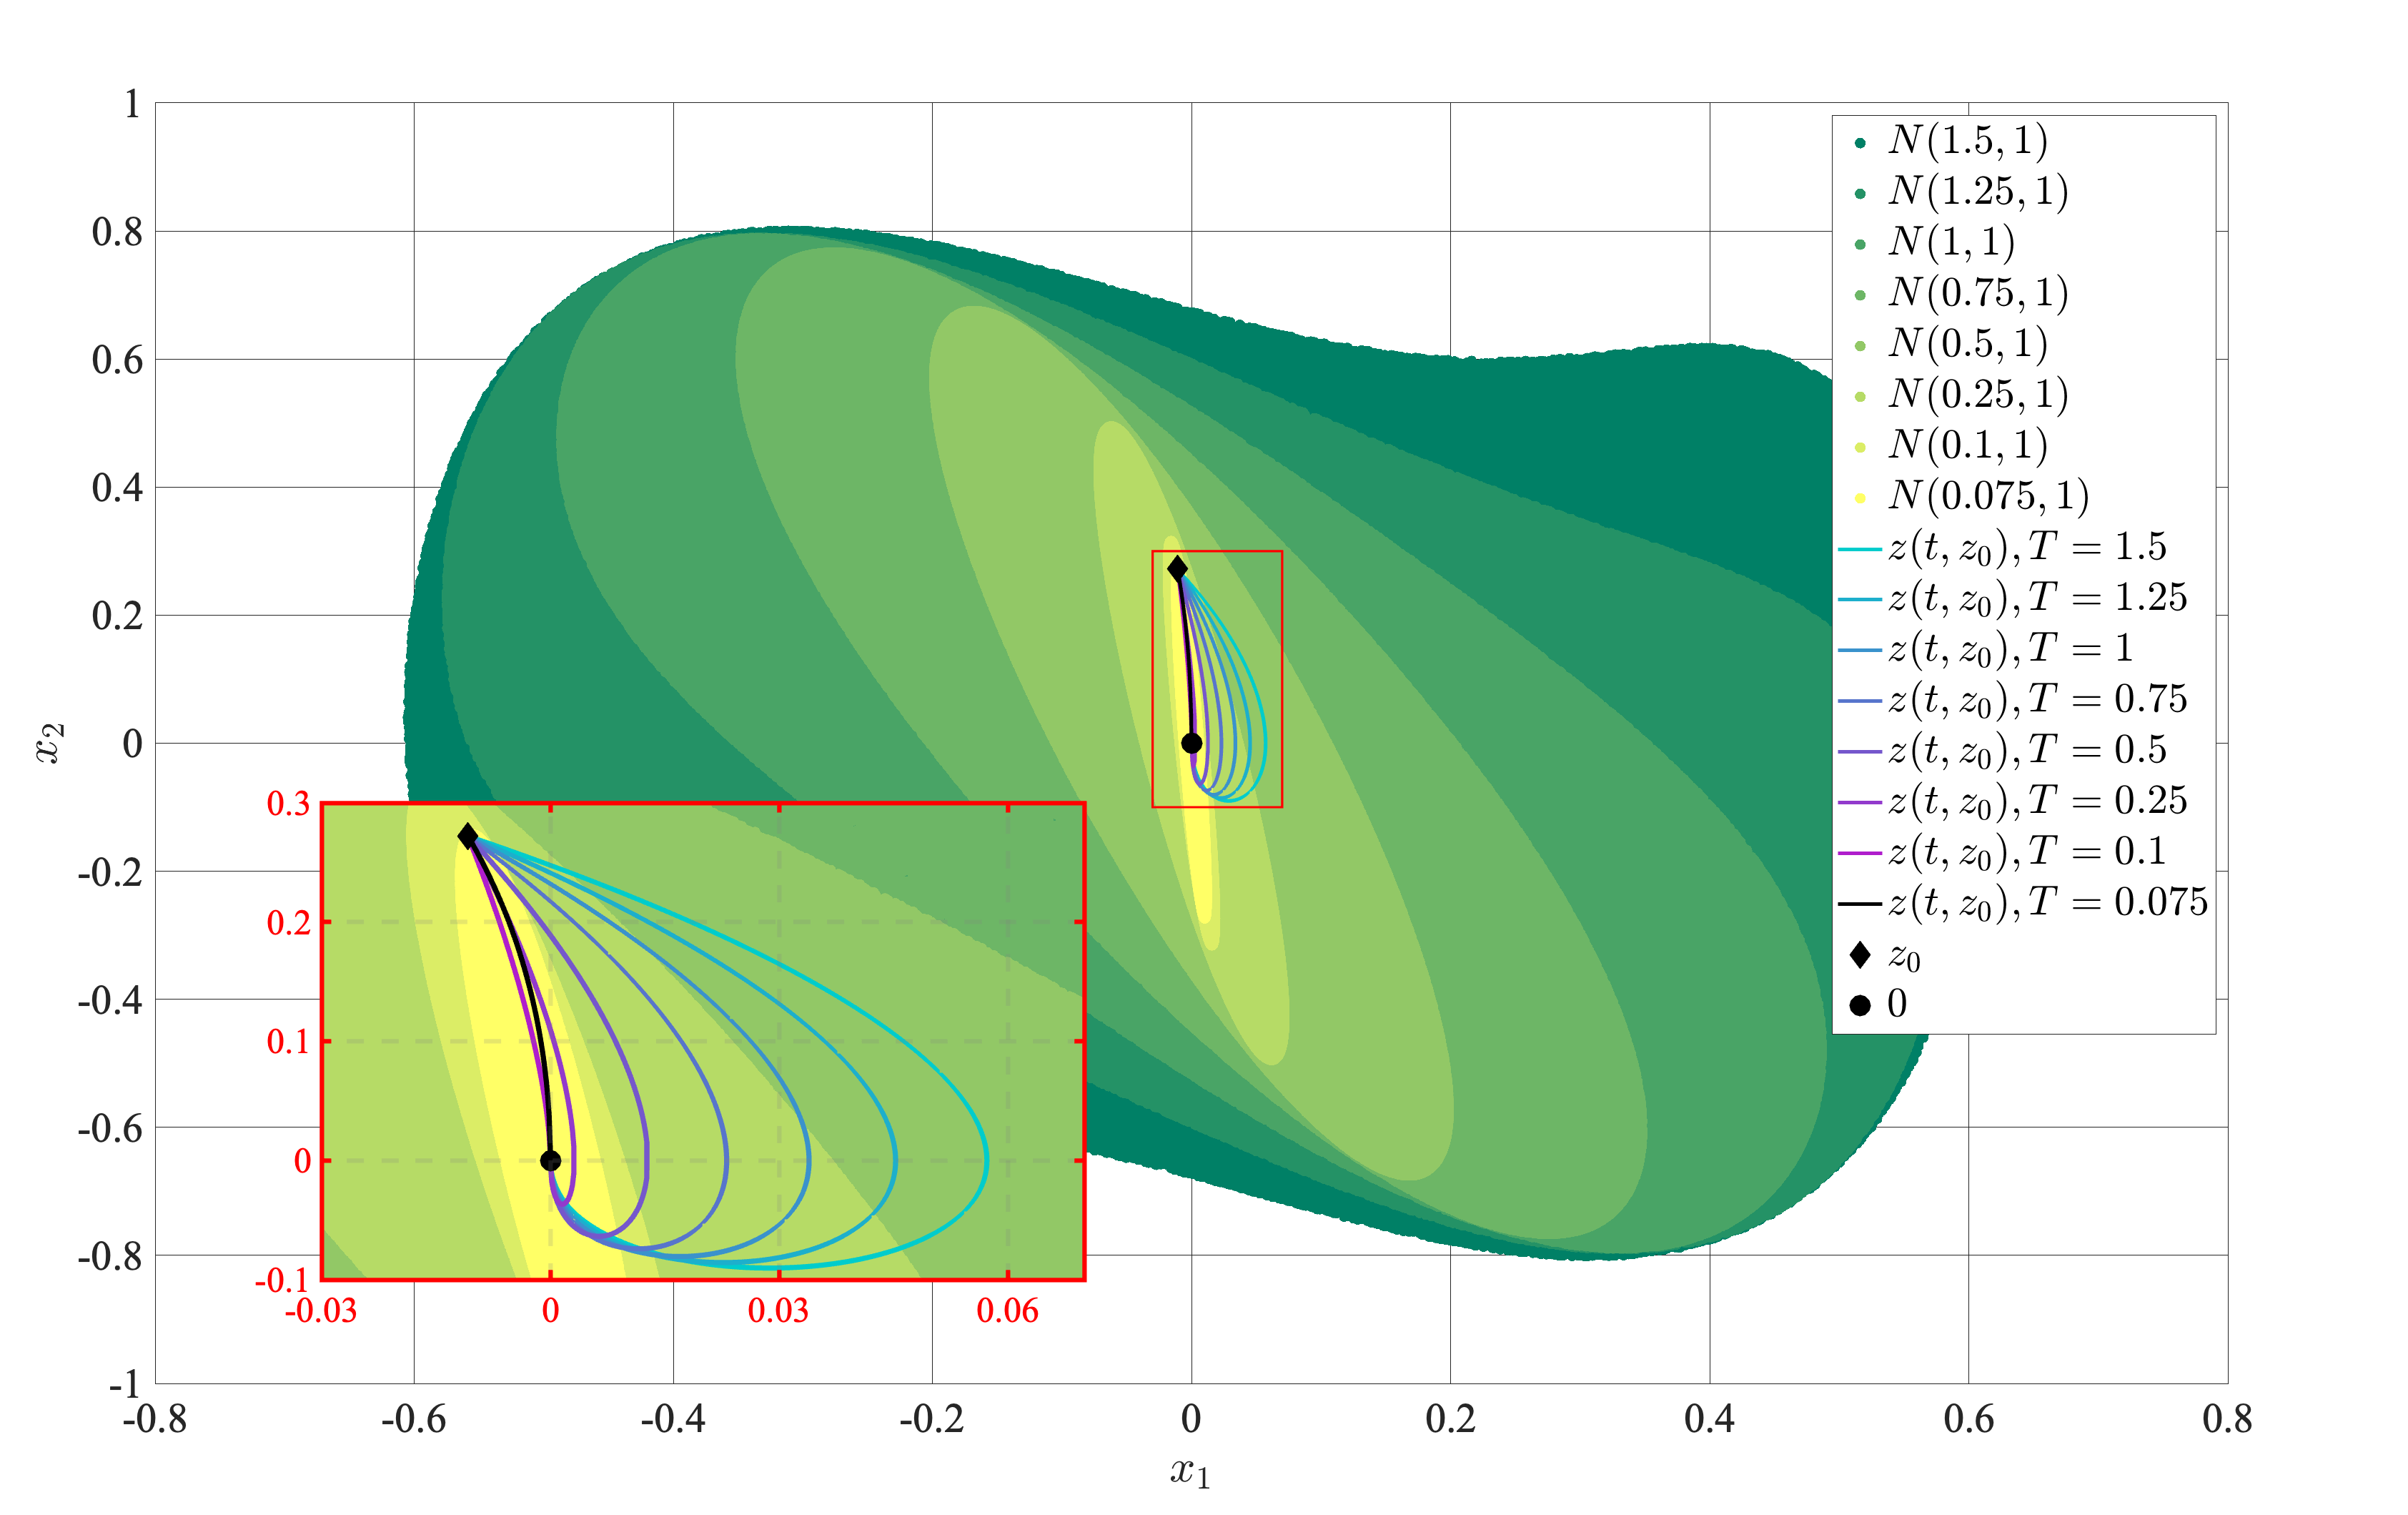
\includegraphics[width=\linewidth]{images/GusevMIOsipov_Duffing_fixed_z0.eps}
    \caption{Результаты экспериментов с переменным $T$.}
    \label{fig:series1}
\end{figure}

Несмотря на то, что условие $z_0 \in B(0,r_1(T))$ Теоремы \ref{th:tends_to_zero} не выполняется при $r_1(T)$, используемом в доказательстве, траектории по-прежнему стремятся к нулю. 
Это можно объяснить слишком строгим выбором $r_1(T)$ и тем, что теорема \ref{th:tends_to_zero} формулирует только достаточные условия для того, чтобы траектории стремились к нулю. 
Можно заметить, что в случае фиксированных начальных условий с уменьшением $T$ относительная разность функционалов $\Delta_J$ уменьшается, что следует из оценки, полученной в теореме \ref{th:functional_error_estimate}.

Теперь мы немного изменим условия эксперимента. 
Мы изменим не только $T$, но и начальные условия $z_0$ так, чтобы, во-первых, выполнялось равенство 
$z_0^{\top} Q_T(0) z_0 = 1$, а во-вторых, чтобы точка $z_0$ находилась внутри 
соответствующего множества нуль-управляемости $G_{-}(T,1)$.


\begin{table}
\caption{Результаты экспериментов с изменением $T$ и $z_0$}
\label{ExampleTable2}
\begin{center}
\begin{tabular}{c|c|c|c|c|c|c}
     № &    $T$  & $z_0$            & $\|z_0\|^2$&$z_0^{\top} Q_T(0) z_0$ &$J(T,z_0)$&$\Delta_J$ \\ \hline 
     1 &   1.500 & [-0.594;-0.057]  & 0.356680   & 0.999993    & 1.075833 & 0.0758407 \\ \hline
     2 &   1.250 & [-0.578;0.226]   & 0.385032   & 0.999997    & 1.110464 & 0.1104671 \\ \hline
     3 &   1.000 & [-0.502;0.508]   & 0.509514   & 0.999999    & 1.108159 & 0.1081607 \\ \hline
     4 &   0.750 & [-0.354;0.652]   & 0.550391   & 1.000000    & 1.048784 & 0.0487844 \\ \hline
     5 &   0.500 & [-0.195;0.638]   & 0.445513   & 1.000000    & 1.009848 & 0.0098475 \\ \hline
     6 &   0.250 & [-0.069;0.481]   & 0.236487   & 1.000000    & 1.000349 & 0.0003490 \\ \hline
\end{tabular}
\end{center}
\end{table} 

Результаты этой серии экспериментов 
показаны на рисунке \ref{fig:series2} и в таблице 
\ref{ExampleTable2}.
Зелеными областями обозначены множества нуль-управляемости $G_{-}(T,1)$ системы 
\eqref{Duffing} при $T = \{0.25, 0.5, 0.75, 1.0, 1.25, 1.5\}$, пунктирные линии 
линии показывают границы множества нуль-управляемости линеаризованной системы 
\eqref{LinearDuffing}, сплошные линии показывают траектории нелинейной системы 
при различных $T$. 
Символы "$\blacklozenge$" разных цветов обозначают 
начальные условия $z_0$, а "$\bullet$" --- целевую точку, расположенную в 
в начале координат. 

Замечание о невыполнении условия из первой части примера актуально и здесь. 
Из таблицы \ref{ExampleTable2} видно, что значения $\Delta_J$ также уменьшаются с уменьшением $T$, но это уменьшение не монотонно. 
По-видимому, это связано с тем, что меняется не только $T$, но и $z_0$.

\begin{figure}
    \centering
    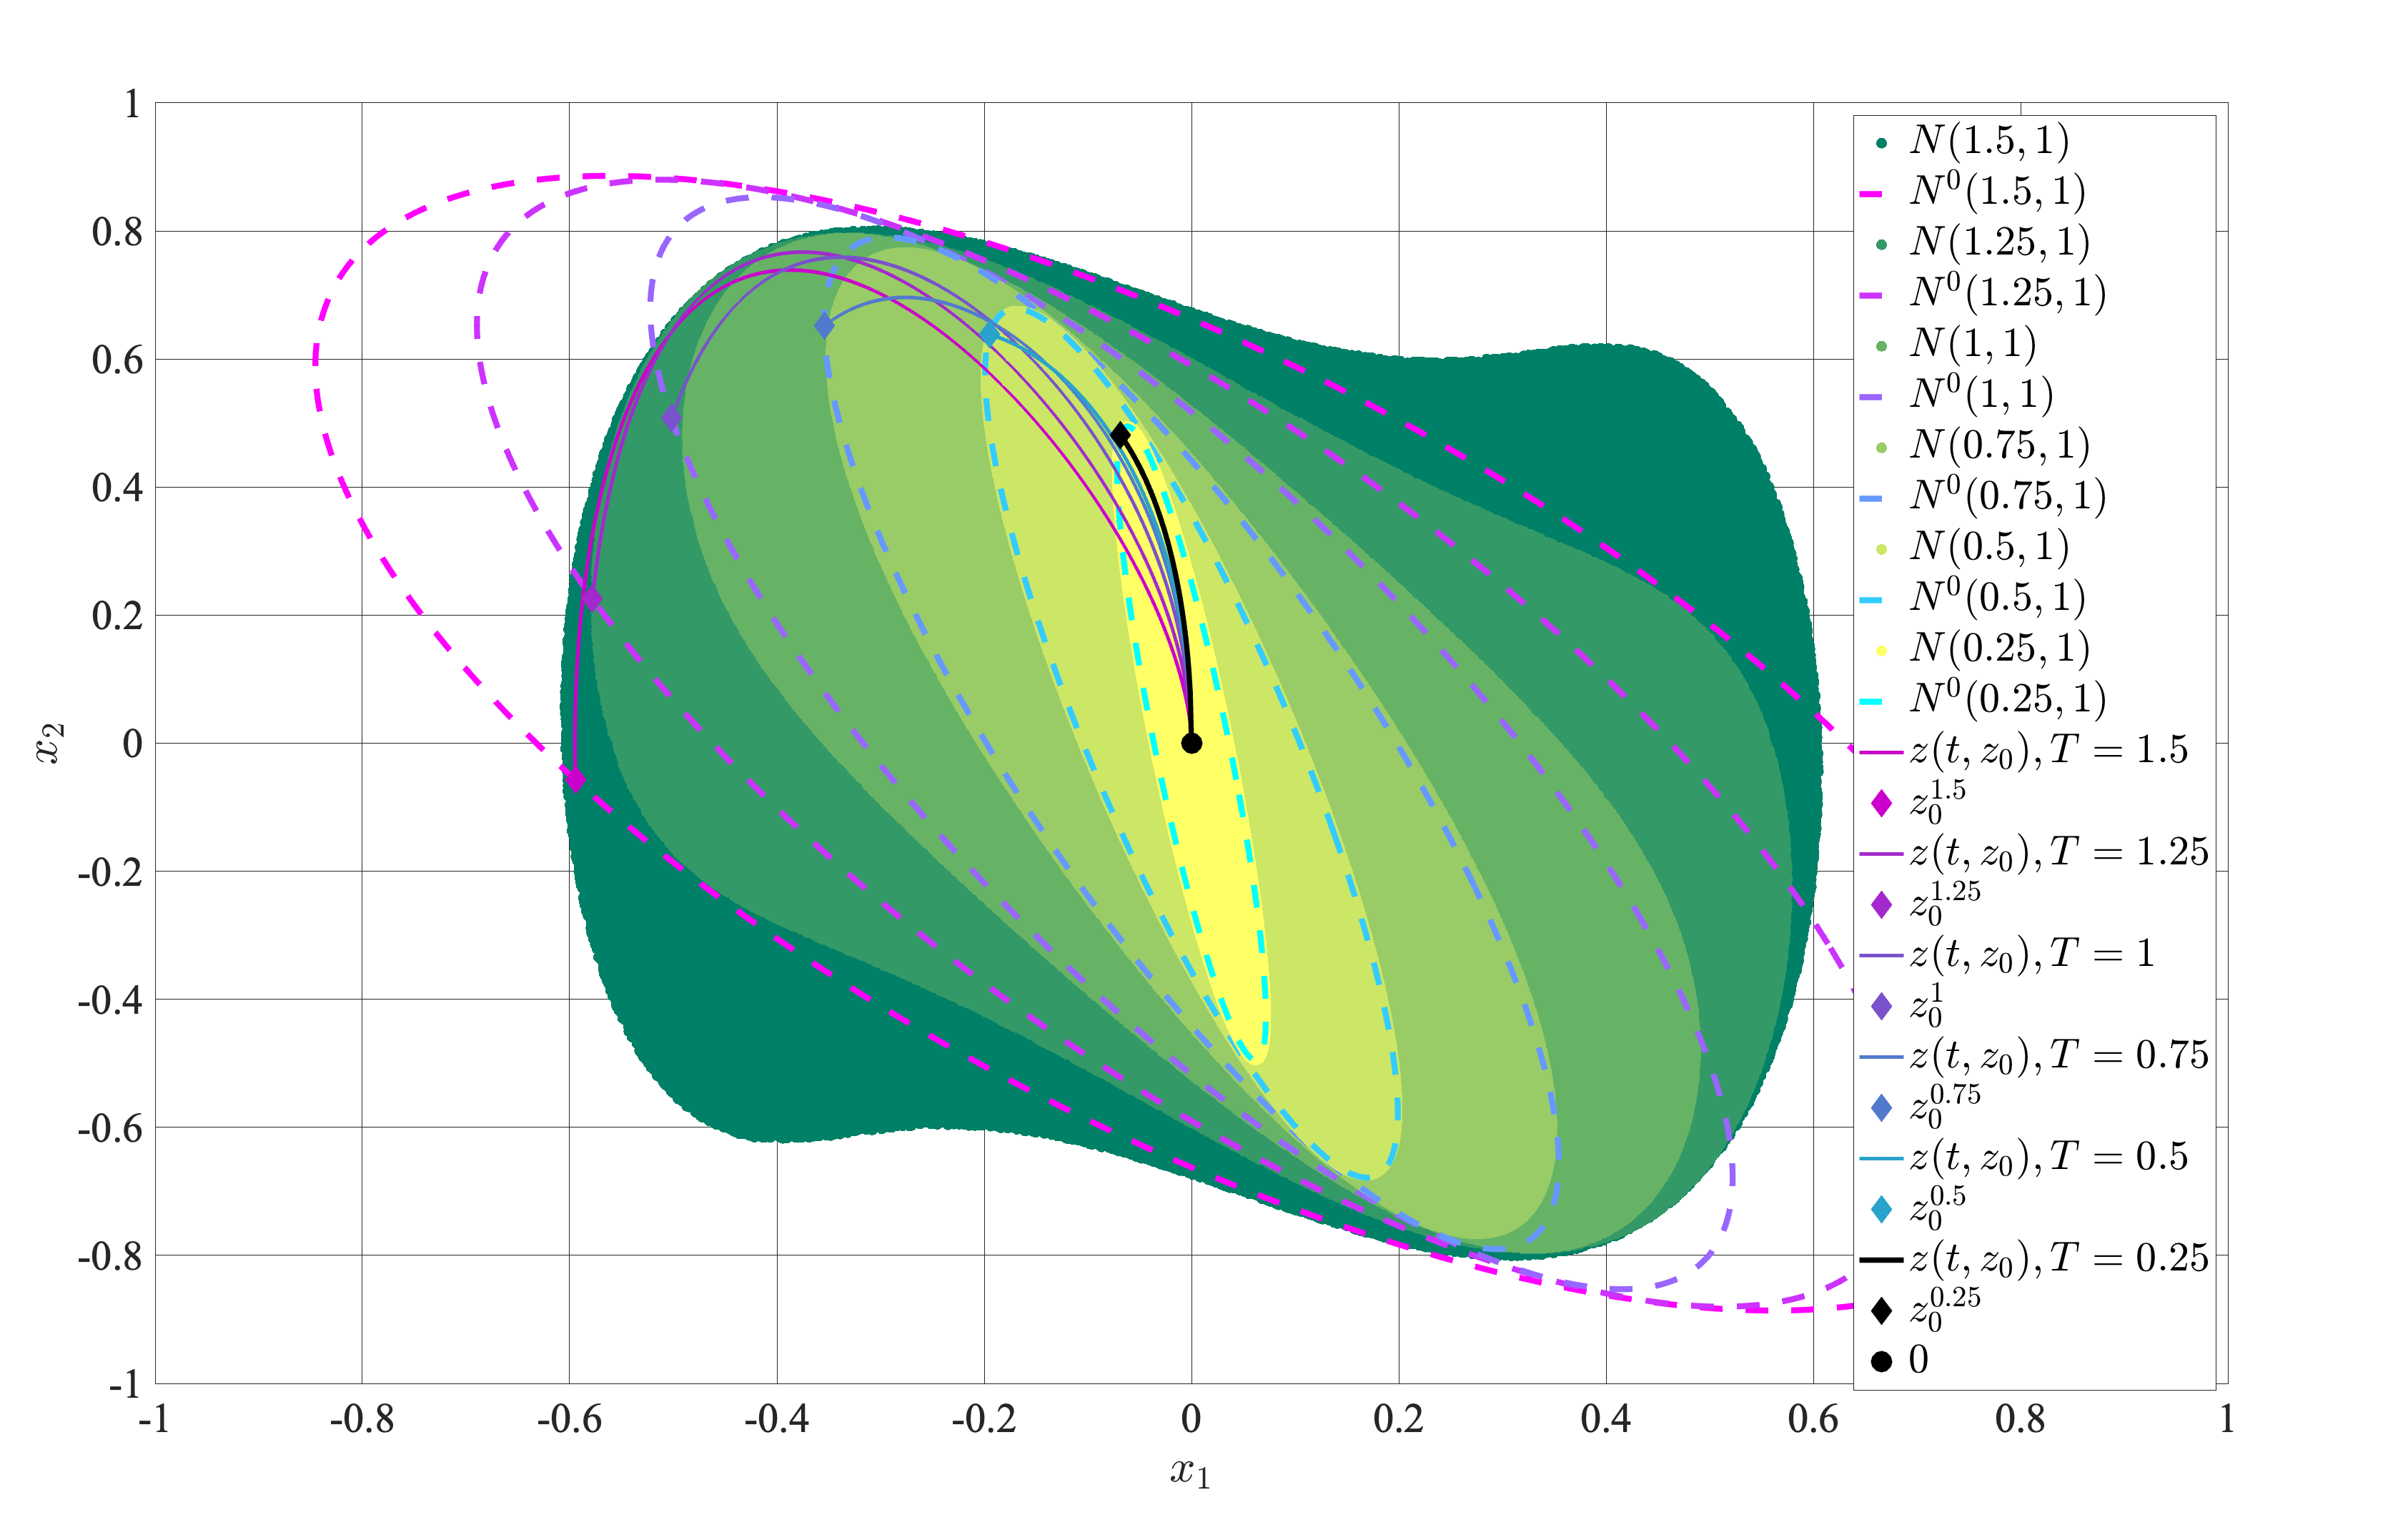
\includegraphics[width=\linewidth]{images/GusevMIOsipov_Duffing_variable_z0.eps}
    \caption{Результаты экспериментов с изменением $T$ и $z_0$}
    \label{fig:series2}
\end{figure}

Также на рисунке \ref{fig:series2} видно, что множества нуль-управляемости нелинейной и линеаризованной систем близки по форме при $ T \leqslant 0.75$. 

\subsubsection{Заключение}
Показано, что метод линеаризации может быть применен к задаче синтеза оптимального управления на конечном интервале времени. 
Линейная обратная связь, расчитанная для линеаризованной системы, также обеспечивает локальное решение задачи синтеза для нелинейной системы, если промежуток времени достаточно мал.   
Для этого требуются достаточно строгие ограничения на асимптотику грамиана управляемости, которые совпадают с достаточными условиями, обеспечивающими асимптотическую эквивалентность множеств достижимости (множеств нуль-управляемости). 
При этих условиях получена оценка для относительных значений погрешности интегрального функционала. 
Для демонстрации реализации описанного метода синтеза приведен пример нелинейной упругой системы под действием внешней силы. 

\end{document}